\subsection{OPTICS}
\label{subsec:opticsresults}

\begin{figure}[ht!]
    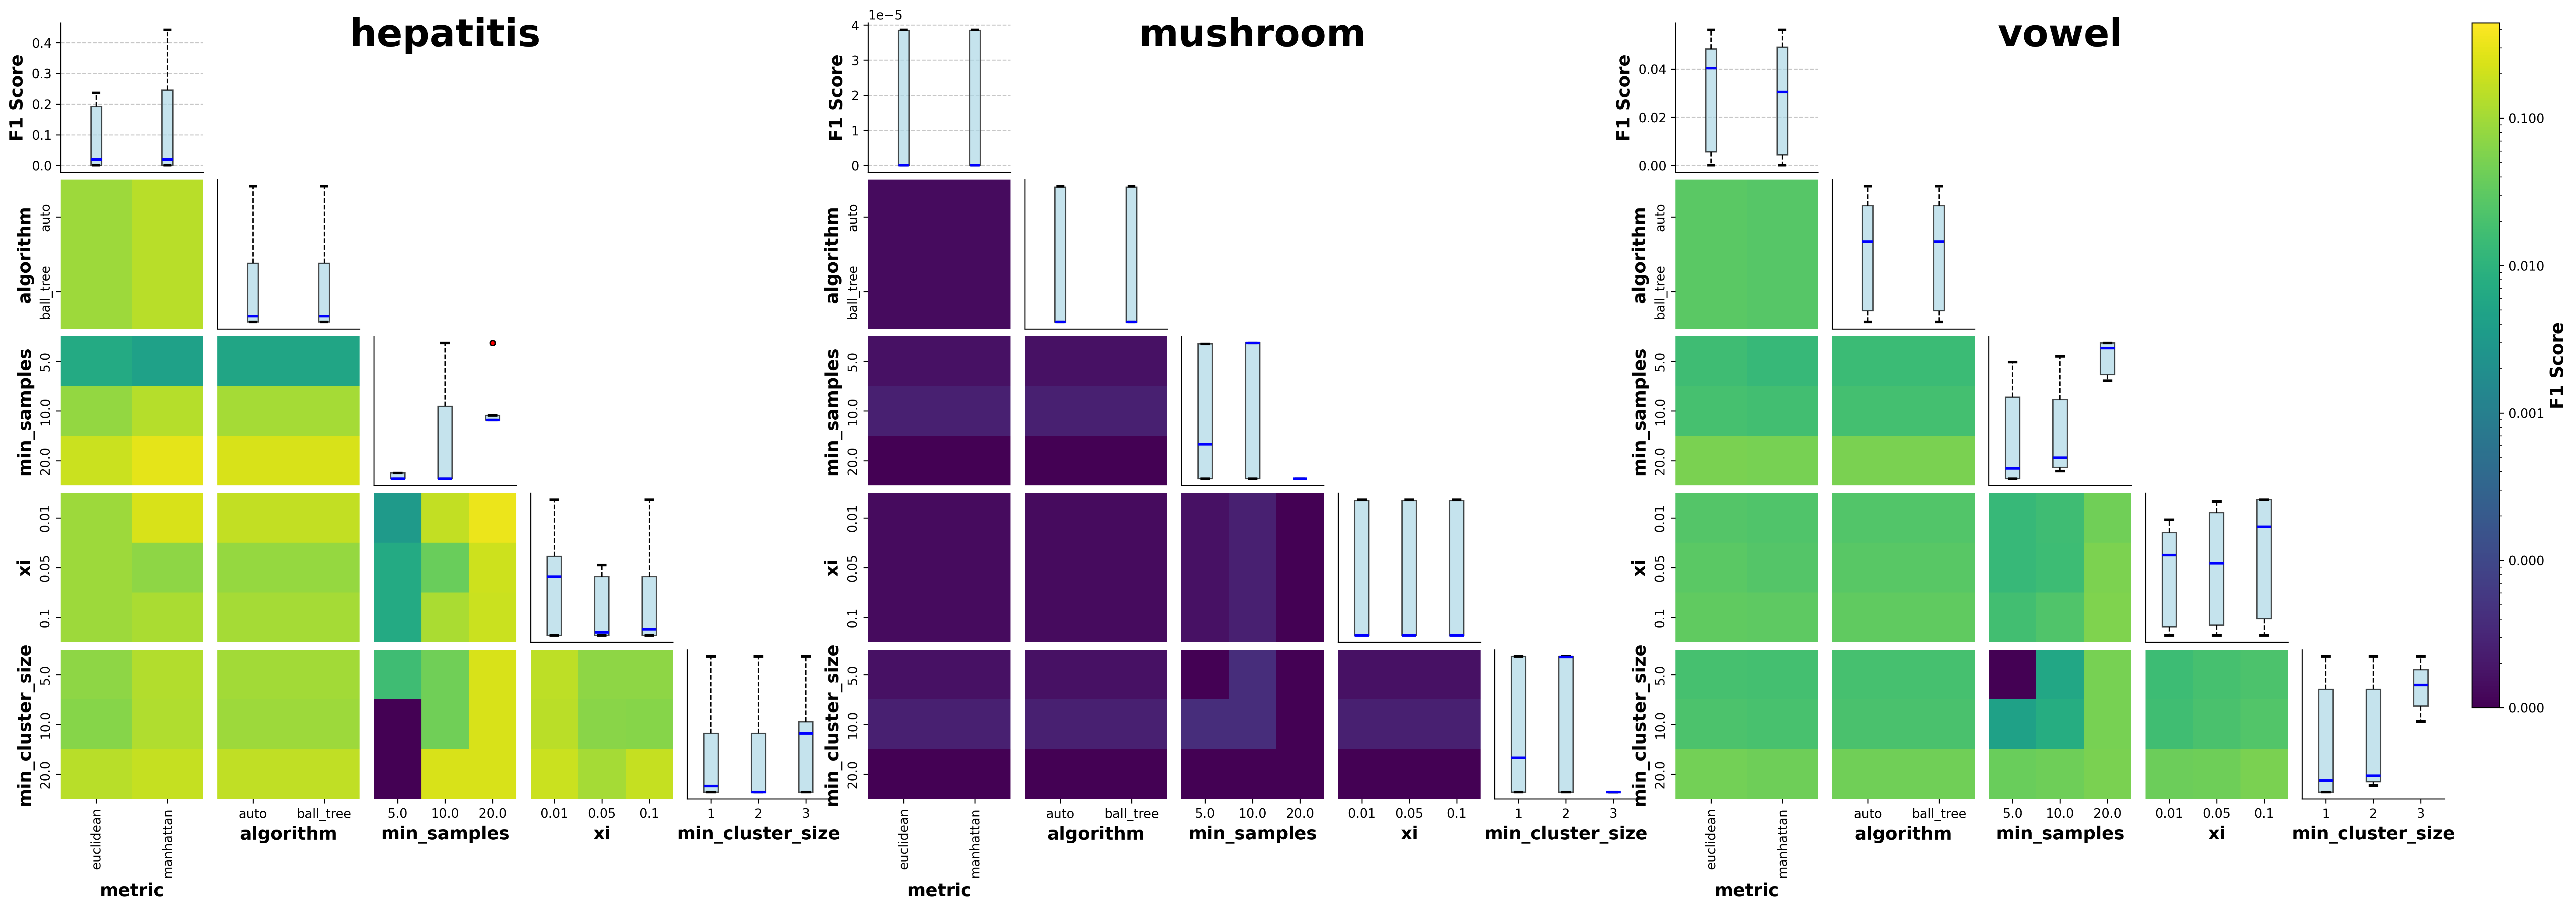
\includegraphics[width=0.5\textwidth]{figures/interactions_optics.png}
    \caption{Parameter interactions for OPTICS}
    \label{fig:interactions_optics}
    \end{figure}

OPTICS demonstrated varying performance across the three datasets. For Hepatitis, it achieved moderate results with an F-measure around 0.23 at optimal parameters. The Mushroom dataset showed very poor performance with F-measures near 0, despite its simpler binary classification nature. The Vowel dataset achieved F-measures around 0.05, which while low, was better than the Mushroom results.

As shown in Figure \ref{fig:interactions_optics}, the algorithm's performance was significantly influenced by parameter choices. The $min\_samples$ parameter had the strongest effect across all datasets, while the $xi$ parameter showed notable impact particularly on the Hepatitis dataset. The metric choice (euclidean vs manhattan) and algorithm implementation (auto vs ball\_tree) had relatively minor effects on the results.

The $min\_cluster\_size$ parameter demonstrated interesting interactions with other parameters, particularly visible in the Hepatitis dataset where higher values generally led to better F-measures when combined with appropriate $min\_samples$ settings. This suggests that OPTICS performs better when allowed to form larger, more stable clusters rather than numerous small ones.

